\documentclass[11pt,a4paper,twoside,openright]{article}  
%alt: [11/12pt,a4paper/letterpaper,oneside/twoside,openany/openright]{book/memoir}
\usepackage{graphicx}

\title{Calculus of Complex Zonotopes}
\author{Santosh Arvind Adimoolam}
\date{}

\begin{document}

\maketitle Models of hybrid systems, that describe the system dynamics
as an interaction between continuous and discrete variables, pose a
significant challenge for formal verification.  Verification of some
of the properties of these systems, like safety and stability, usually
requires computing the set of reachable states of the system.  For a
general class of these models that have differential equations and
discrete modes for switching, exact computation of the reachable set
is undecidable~\cite{todo}, except in particular cases.  Even in a
simpler case like a discrete time affine hybrid system, the exact
reachable set at any given time is a union of exponential number of
convex sets in the number of time steps.  Instead, we can find a
sufficiently accurate over-approximation of the infinite set of
reachable states.  To do so, we need to represent an infinite set of
states symbolically by a {\it set representation}, which can be
efficiently manipulated for the computation of the desired
over-approximation.  Some examples of a set representation are {\it
  convex polyhedron}, represented by either linear
inequalities~\cite{cousot1978automatic,Sankaranarayanan+Dang+Ivancic-08-Symbolic}
or a convex hull of a finite set of points~\cite{kvasnica2004multi};
{\it
  ellipsoid}~\cite{DBLP:journals/tecs/AllamigeonGSGP16,kurzhanskiy2006ellipsoidal},
represented by a positive semi-definite matrix and a center; {\it polynomial
  sub-level sets}~\cite{DBLP:conf/esop/AdjeGG10,prajna2004safety} ;
etc.  In numerical abstract interpretation, a set representation is
usually an {\it abstract domain}, which is a lattice with an
abstraction and a concretization map~\cite{jeannet2009apron}.

\section{Problem and related work}
We consider the problem of efficiently computing a sufficiently
accurate over-approximation of the unbounded time reachable set that
is useful for verifying properties like invariance and stability.  The
unbounded time reachable set is usually approximated as a {\it
  positive invariant}, which is a set of states whose next set of
reachable states is contained within itself.  The potentiality of a
set representation for efficient computation of a positive invariant
of a hybrid system is affected by the following characteristics.  (i)
Closure of the set representation under set operations like linear
transformation, Minkowski sum, intersection and inclusion-checking,
etc, and efficient computation of the same.  (ii) Existence of a
positive invariant for the system that can be encoded by the set
representation. (iii) Efficient encoding of the positive invariant by
the set representation.  Well known set representations for computing
reachable sets have some of the above characteristics, but not all.
For example, polytopes have the advantage that they are closed under
linear transformation, Minkowski sum and intersection and for a stable
linear transformation, there exists a polytopic invariant.  However,
the Minkowski sum operation is costly because it can lead to a
quadratic increase in the number of vertices and an exponential
increase in the number of faces.  Also, the number of faces of a
polytopic positive invariant for a stable linear system can be
arbitrarily large.  Ellipsoids have the advantage that they are closed
under linear transformation and can also efficiently represent the
positive invariant of a stable linear transformation.  But ellipsoids
are not closed under Minkowski sum.  Recently work computes the
over-approximation of the Minkowski sum of ellipsoids by a minimum
volume ellipsoid~\cite{}.  Still, there can be significant
approximation error in the ellipsoidal approximation of the Minkowski
sum.


\paragraph{Real zonotope, its usefulness and drawback.}
Zonotope~\cite{DBLP:conf/hybrid/Girard05} is yet another set
representation, which is specified as a linear combination of real
vectors and a center, such that the absolute values of the combining
coefficients are bounded within unity.  Geometrically, a zonotope is
the Minkowski sum of line segments and hence a type of polytope.
Zonotopes have also been extended to the more general quadratic
zonotopes~\cite{DBLP:conf/aplas/AdjeGW15}, which is a quadratic
function of real valued intervals.  Zonotopes have the advantage that
they are efficiently closed under linear transformation and Minkowski
sum operations.  Therefore, they have been successfully applied to the
computation of bounded time reachable sets of uncertain continuous
linear systems~\cite{todo} and affine hybrid systems with large dwell
time for switching~\cite{todo}.  But for over-approximation of the
unbounded time reachable set by a positive invariant, real zonotopes
have the have the following drawback.  We can not guarantee the
existence of a positively invariant real zonotope for the case of a
stable linear transformation having complex eigenvalues.  When the
eigenvectors of a stable linear transformation are real valued, then
collecting the eigenvectors of the matrix among the generators of the
zonotope gives a positive invariant.  However, this result does not
hold when the eigenvectors have complex values, i.e., have non-zero
imaginary and real parts.



\section {Contribution}
\paragraph{Complex zonotope.}  To address the above drawback of real
zonotopes, we extend them to the complex valued domain to yeild a set
representation called {\it complex zonotope}.  A basic representation
of the complex zonotope is a linear combination of complex valued
vectors with complex combining coefficients, whose absolute values are
bounded within unity.  We show that a complex zonotope captures
contraction along the complex valued eigenvectors of a linear
transformation, which relates to existence of a positively invariant
complex zonotope.  The real projection of a complex zonotope can
represent not only Minkowski sums of line segments, but also some
ellipsoids.  Hence, they can represent non-polyhedral sets as well as
polytopic zonotopes.  They are different from quadratic
zonotopes~\cite{DBLP:conf/aplas/AdjeGW15xs}, because while the latter is
a quadratic function of real valued intervals, a complex zonotope is a
complex linear combination of circles in the complex plane.
%
\begin{figure}
  \begin{minipage}{0.5\textwidth}
    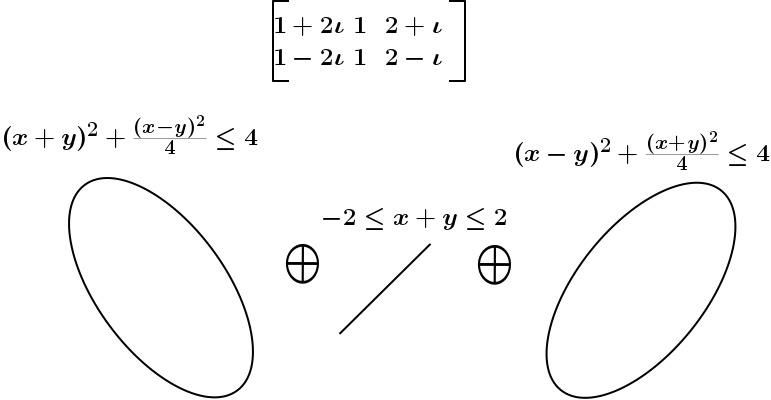
\includegraphics[scale=0.6]{figures/complex-zonotope.png}
  \end{minipage}
  %
  \hspace{5em}
  %
  \begin{minipage}{0.4\textwidth}
    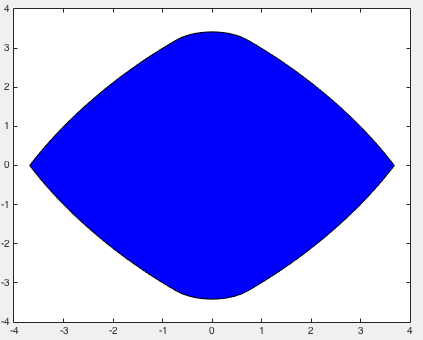
\includegraphics[scale=0.3]{figures/CZhull.png}
  \end{minipage}
  %
  \caption{Figure of a complex zonotope}
\end{figure}
%
\paragraph{Template complex zonotope.}  In order to easily refine a
complex zonotope by adding arbitrary generators while approximating a
given set, we introduce the {\it template complex zonotope}
representation.  In a template complex zonotope, the absolute values
of combining coefficients have variable bounds called scaling factors.
The scaling factors can be adjusted to find better over-approximations
while adding arbitrary generators in a {\it template}.  Just like
simple zonotopes, template complex zonotopes are also efficiently
closed under linear transformation and Minkowski sum operations.  But
in addition, template complex zonotope can easily represent a positive
invariant for a linear transformation based on the eigenstructure of
the matrix, as described previously.  We propose a sufficient
condition for checking inclusion between template complex zonotopes,
expressed as a set of second-order conic (convex) constraints on the
scaling factors and other auxiliary variables.  This condition is
useful in practice, which we demonstrate through our experiments in
safety and stability verification on some benchmark examples.

\paragraph{Augmented complex zonotope.}  Template complex
zonotopes are not closed under intersection with sub-level sets of
linear inequalities.  This is also a drawback of real zonotopes.
Previous work addressed this drawback for real zonotopes by allowing
linear constraints on the combining coefficients, in a more general
representation called {\it constrained
  zonotopes}~\cite{scott2016constrained}.  But if we emulate this
approach for complex zonotopes, we get linear constraints on the
complex valued combining co-coefficients in addition to the quadratic
absolute value bounds.  However, for the resultant set representation
having quadratic absolute value constraints as well as linear
constraints, the problem of finding a reasonable convex-relaxation for
inclusion-checking, that works well in practice, seems intractable.
Instead, we define a different representation called {\it augmented
  complex zonotope}, which is geometrically equivalent to a complex
zonotope, but whose representation allows efficient computation of a
non-trivial over-approximation of the intersection with a class of
linear constraints.  The over-approximation is computed as a simple
algebraic expression of the parameters of the augmented complex
zonotope.  In the course of the derivation of this result, we also
find a general mathematical result about intersection of Minkowski sum
of convex sets with another convex set.

\paragraph{Unbounded time safety verification.}
We express operations on augmented complex zonotopes like linear
transformation, Minkowski sum, over-approximation of intersection with
constraints and support of a vector as affine expressions of some of
the specification parameters.   We also derive a second order conic
program for checking inclusion between two augmented complex
zonotopes.  Henceforth, we derive a second order conic
program for checking the safety of an affine hybrid system.  The fact
that a complex zonotope can both capture the contraction along complex
eigenvectors and also efficiently represent linear transformation and
Minkowski sum makes it an efficient set representation for unbounded
time safety verification.  We demonstrate the efficiency of the safety
verification approach by implementing on some benchmark examples.

\paragraph{Stability verification of nearly periodic linear impulsive
  systems.}  %% The specification of an augmented complex
%% zonotope has a complex matrix, called {\it primary template}, a real
%% matrix called {\it secondary template}, the center of the constituting
%% template complex zonotope, called {\it primary offset}, bounds on the
%% absolute values of the complex combining co-efficients, called {\it
%%   scaling factors} and the {\it lower and upper interval bounds} on
%% the real combining co-efficients.
 %% These
%% expressions are affine functions of the primary offset, scaling
%% factors and lower and upper interval bounds. 
  Our analysis of template complex zonotopes for the case of discrete
  time switched linear systems is extended to verify stability of {\it nearly
    periodic linear impulsive systems}.  We first derive bounds on the
  amount of contraction of a complex zonotope after a linear
  transformation.  Then we derive a second order conic program to
  synthesize a contractive complex zonotope for a collection of linear
  transformations.  We apply these results to verify the exponential
  stability of nearly periodic linear impulsive systems.  We implement
  the procedure on some benchmark examples to demonstrate its
  efficiency.

\section {Organization}
The dissertation contains five main chapters and a conclusive chapter.
In Chapter 1, we briefly discuss the use of set representation for
computing reachable sets of hybrid systems and the desirable
characteristics of a good set representation.  In light of these
characteristics, we provide a short review of some set representations
that discusses their advantages and drawbacks.  Then we review
simple/real zonotopes and the commonly used operations on them in
reach set computation.  We also review the definitions polynomial and
constrained zonotopes, which are previously known extensions of the
simple zonotope.  Then we shall describe the shortcoming of the real
zonotope in computing a positive invariant.

In Chapter 2, we introduce the complex zonotope set representation
that addresses the drawback of real zonotope described in the previous
chapter.  We define the basic representation of a complex zonotope and
state a result about how a complex zonotope can efficiently represent
a positive invariant for a stable linear transformation based on the
eigenstructure.  Next we define the more general template complex
zonotope representation, which permits a way of refining a complex
zonotope while approximating a given set.  We discuss operations on
template complex zonotopes that are used in reach set computation and
derive a second order conic program for checking inclusion between
template complex zonotopes.  Using the results, we derive a second
order conic program for unbounded time safety verification of linear
systems and illustrate it with an example.

In Chapter 3,
we introduce augmented complex zonotopes for computing non-trivial
intersection with a class of sub-level sets of linear inequalities
called sub-parallelotopes.  Apart from the intersection, we discuss
other operations on augmented complex zonotope used in the computation
of reachable sets.  Also, we state a second order conic program for
checking inclusion between augmented complex zonotopes.

In Chapter 4, we apply augmented complex zonotopes for unbounded time
safety verification of affine hybrid systems.  We derive a second
order conic program for checking safety, which is based on computing a
suitable positively invariant augmented complex zonotope.  We
implement the approach on some benchmark examples to demonstrate its
efficiency.

In Chapter 5, we apply template complex zonotopes for verifying
exponential stability of linear impulsive systems with sampling time
uncertainty.  We discuss a procedure for stability verification, which
consists of synthesizing a possibly contractive template complex
zonotopes and verifying their contraction.  We implement this
procedure on some benchmark examples to demonstrate its efficiency.

The concluding remarks are stated in Chapter 6.








\bibliographystyle{plain}
\bibliography{PhdThesis/myLib}





\end{document}
